%%%%%%%%%%%%%%%%%%%%%%%%%%%%%%%%%%%%%%%%%
% Jacobs Landscape Poster
% LaTeX Template
% Version 1.0 (29/03/13)
%
% Created by:
% Computational Physics and Biophysics Group, Jacobs University
% https://teamwork.jacobs-university.de:8443/confluence/display/CoPandBiG/LaTeX+Poster
% 
% Further modified by:
% Nathaniel Johnston (nathaniel@njohnston.ca)
%
% This template has been downloaded from:
% http://www.LaTeXTemplates.com
%
% License:
% CC BY-NC-SA 3.0 (http://creativecommons.org/licenses/by-nc-sa/3.0/)
%
%%%%%%%%%%%%%%%%%%%%%%%%%%%%%%%%%%%%%%%%%

%----------------------------------------------------------------------------------------
%	PACKAGES AND OTHER DOCUMENT CONFIGURATIONS
%----------------------------------------------------------------------------------------

\documentclass[final]{beamer}

\usepackage[scale=1.24]{beamerposter} % Use the beamerposter package for laying out the poster

\usepackage{tikz}
\usepackage{todonotes}
\usepackage{epstopdf}
\epstopdfsetup{suffix = {}}
\usepackage{hyperref}
\usepackage{subfigure}  % Written by Steven Douglas Cochran
\usepackage{amssymb,amsmath,bm}    % From the American Mathematical Society
\usepackage{siunitx} % for units like degree, ...
\sisetup{unitsep=\cdot,binary-units=true}
\usepackage{mathtools}
\usepackage{xcolor,soul}
\usepackage{geometry}
\usetheme{confposter} % Use the confposter theme supplied with this template

\setbeamercolor{block title}{fg=BUred,bg=white} % Colors of the block titles
\setbeamercolor{block body}{fg=black,bg=white} % Colors of the body of blocks
\setbeamercolor{block alerted title}{fg=BUred,bg=gray!70} % Colors of the highlighted block titles
\setbeamercolor{block alerted body}{fg=black,bg=gray!10} % Colors of the body of highlighted blocks


% Many more colors are available for use in beamerthemeconfposter.sty

%-----------------------------------------------------------
% Define the column widths and overall poster size
% To set effective sepwid, onecolwid and twocolwid values, first choose how many columns you want and how much separation you want between columns
% In this template, the separation width chosen is 0.024 of the paper width and a 4-column layout
% onecolwid should therefore be (1-(# of columns+1)*sepwid)/# of columns e.g. (1-(4+1)*0.024)/4 = 0.22
% Set twocolwid to be (2*onecolwid)+sepwid = 0.464
% Set threecolwid to be (3*onecolwid)+2*sepwid = 0.708

\newlength{\sepwid}
\newlength{\onecolwid}
\newlength{\twocolwid}
\newlength{\threecolwid}
\setlength{\paperwidth}{48in} % A0 width: 46.8in
\setlength{\paperheight}{36in} % A0 height: 33.1in
\setlength{\sepwid}{0.022\paperwidth} % Separation width (white space) between columns
\setlength{\onecolwid}{0.22\paperwidth} % Width of one column
\setlength{\twocolwid}{0.464\paperwidth} % Width of two columns
\setlength{\threecolwid}{0.708\paperwidth} % Width of three columns
\setlength{\topmargin}{-0.25in} % Reduce the top margin size
\setlength{\leftmargin}{-0.25in}
\setlength{\rightmargin}{-0.25in}

%-----------------------------------------------------------

\usepackage{graphicx}  % Required for including images

\usepackage{booktabs} % Top and bottom rules for tables
%\usepackage{subfigure}

%-----------------------------------------------------------
% TITLE SECTION
%-----------------------------------------------------------

\title{Smart Control of 2 Degree of Freedom Helicopters} % Poster title

\author{Glenn Janiak, Ken Vonckx, Advisor: Dr. Suruz Miah} % Author(s)


\institute{Department of Electrical and Computer Engineering, Bradley University, Peoria IL} %Institution(s)
\vskip -.5cm

%-----------------------------------------------------------
% POSTER CONTENT
%-----------------------------------------------------------

\begin{document}

\addtobeamertemplate{block end}{}{\vspace*{1ex}} % White space under blocks
\addtobeamertemplate{block alerted end}{}{\vspace*{2ex}} % White space under highlighted (alert) blocks

\setlength{\belowcaptionskip}{2ex} % White space under figures
%\setlength\belowdisplayshortskip{2ex} % White space under equations

\begin{frame}[t] % The whole poster is enclosed in one beamer frame

\begin{columns}[t]

\begin{column}{\sepwid}\end{column} % Empty spacer column

\begin{column}{\onecolwid} % The first column

%-----------------------------------------------------------
% OBJECTIVE AND CONTRIBUTION
%-----------------------------------------------------------

\begin{alertblock}{Objective and Contribution}
%
\textbf{Objective}
\vskip -0.75cm
\begin{itemize}
    \item Develop a platform allowing mobile devices to control the motion of a group of helicopters
\end{itemize}
%\begin{itemize}
%    \item Develop a platform that allows mobile devices to control helicopters with the least amount of error via an embedded system 
%\end{itemize}
%
\vskip -1cm
\textbf{Contribution}
\vskip -0.75cm
\begin{itemize}
    \item Determine trade-offs between traditional control techniques and machine learning
    %\item Embedded System Implementation
    %\item Mobile Device Control 
    \item Multi-Helicopter Application
\end{itemize}
\vskip -0.75cm
\textbf{Applications}
\vskip -0.75cm
\begin{itemize}
    \item Teleoperation approach to search and rescue 
    \item Aerial turbulence resistance 
\end{itemize}

%


\end{alertblock}

%-----------------------------------------------------------
% PROBLEM SETUP
%-----------------------------------------------------------
\vskip -1cm
\begin{block}{Problem Setup}
\vskip -1cm
%\begin{enumerate}
%    \item Develop and linearize system model
%    \item Simulate algorithms in MATLAB
%    \item Test algorithms on desktop computer using USB connection 
%    \item Test algorithms on Raspberry Pi microcontroller
%    \item Test algorithms on mobile device
%\end{enumerate}

\begin{figure}
    \centering
    % \fcolorbox{gray!10}{gray!10}{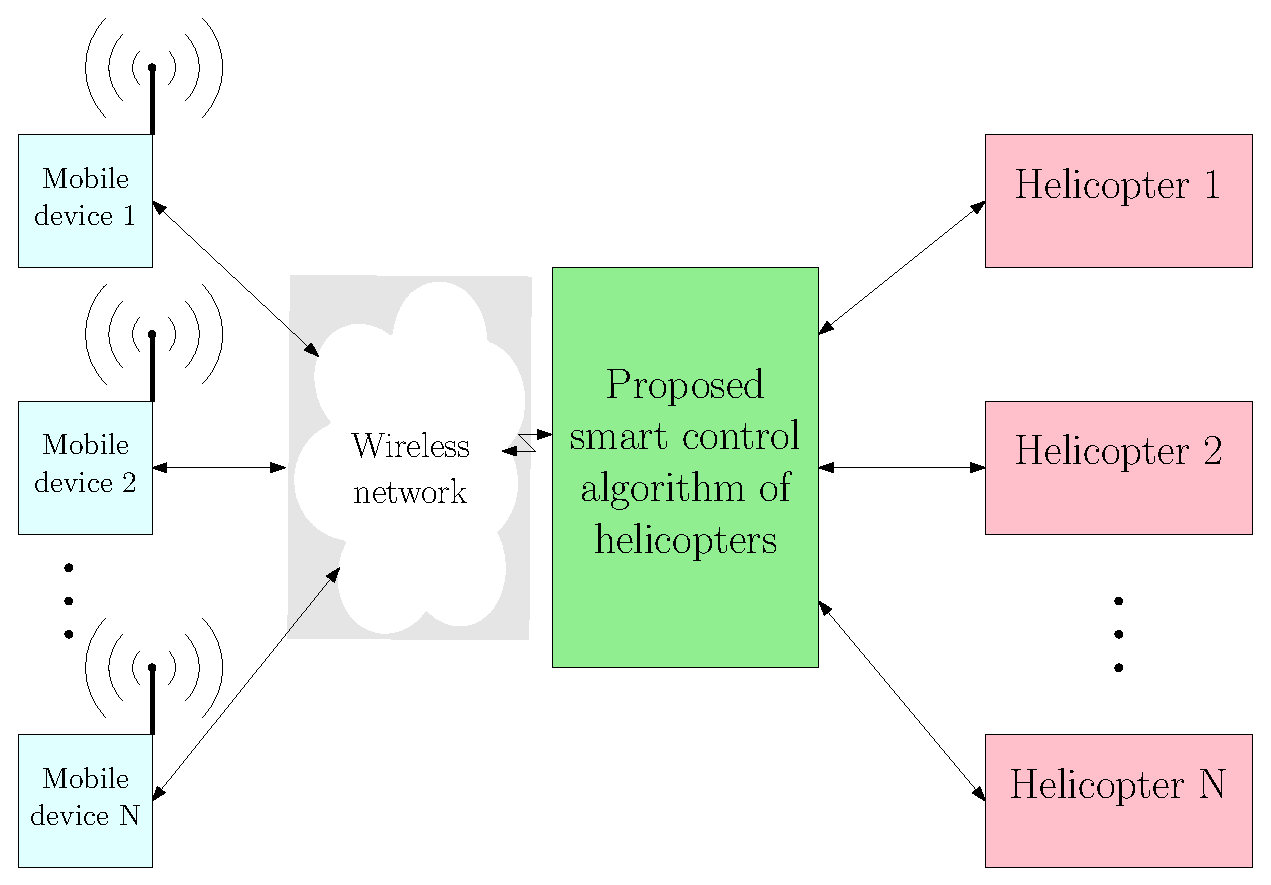
\includegraphics[height=.15\textheight,width=\textwidth,keepaspectratio=true]{figs/ProblemStatementImage_Gray2}}
    \fcolorbox{gray!20}{gray!20}{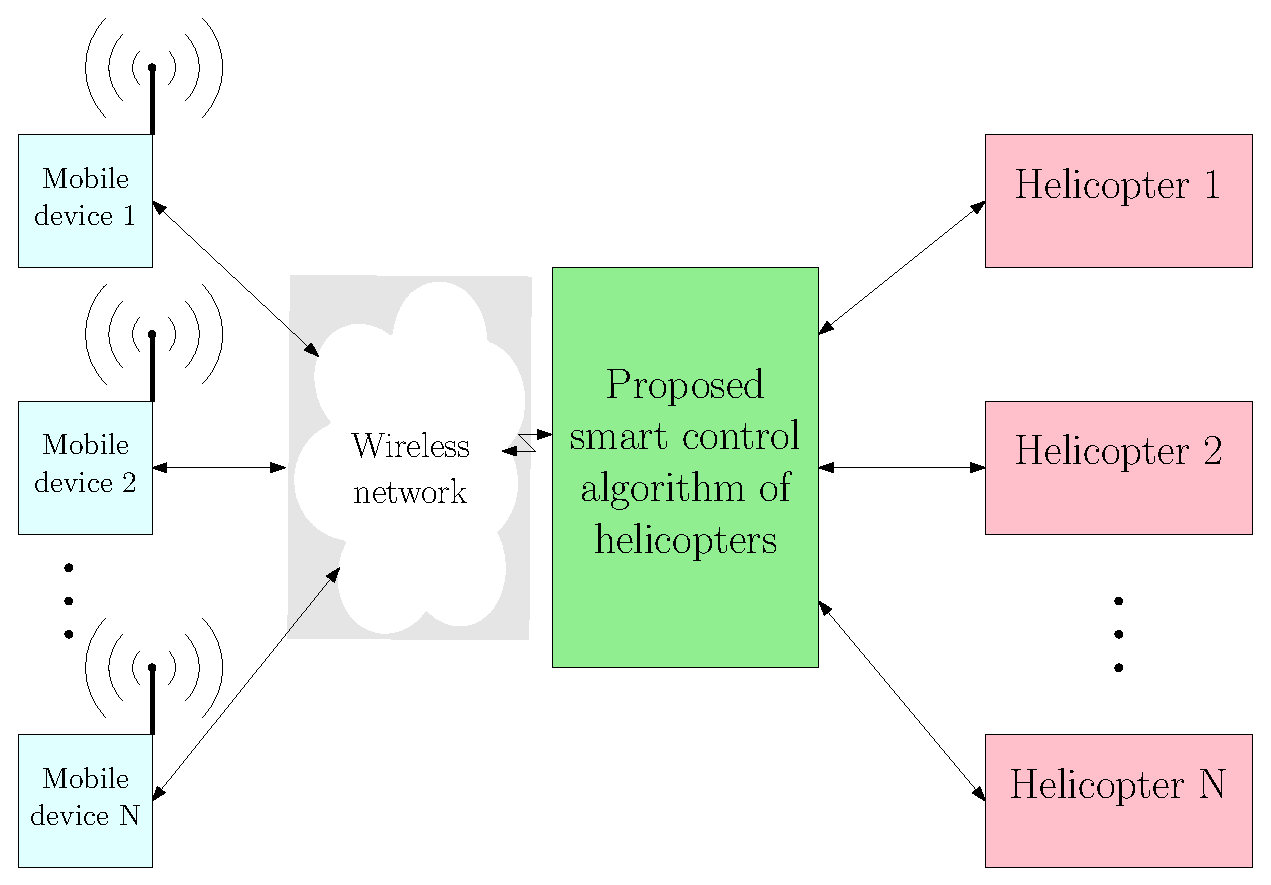
\includegraphics[height=.15\textheight,width=\textwidth,keepaspectratio=true]{figs/ipe/highLevel_gry_grn.eps}
    }
    \caption{High level architecture of the proposed system.}
    \label{fig:highLevelDiagram}
\end{figure}
\begin{figure}
    \centering
    % \missingfigure{Insert figure.}
    \fcolorbox{gray!10}{gray!10}{
    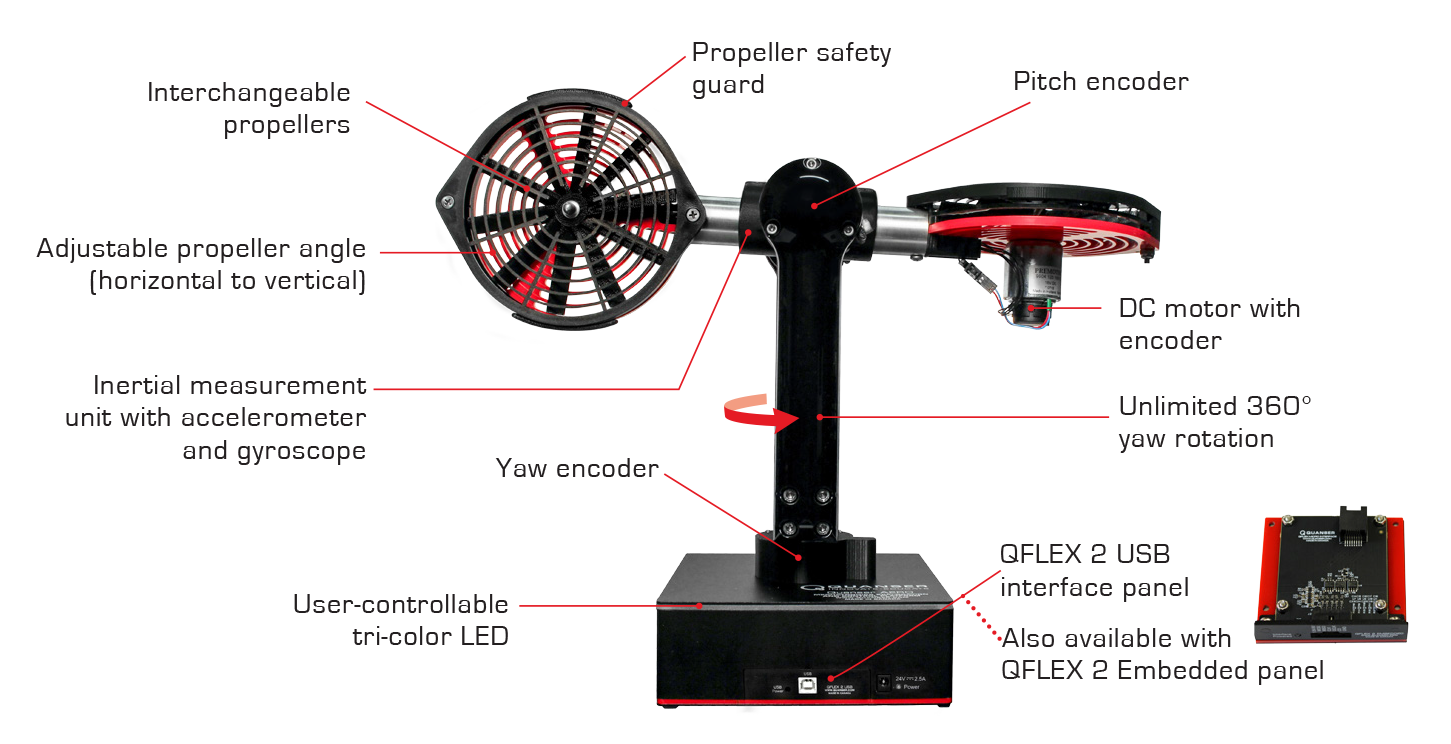
\includegraphics[height=.2\textheight,width=.92\textwidth,keepaspectratio=true]{figs/img/quanserAero.png}
    }
    \caption{2-DOF helicopter (Quanser Aero).}
    %\caption{DC motors are attached to main and tail rotors which allow the helicopter to change its pitch and yaw respectively.}
    \label{fig:helicoterModel}
\end{figure}
\vskip -1cm
$\bullet$ State-space representation of 2-DOF helicopter
\begin{align*}
\begin{bmatrix}
    \dot\theta\\
    \dot\psi\\
    \ddot{\theta}\\
    \ddot{\psi}
\end{bmatrix}&=
%\label{eq:matrixA}
\begin{bmatrix}
    0 & 0 & 1 & 0 \\
    0 & 0 & 0 & 1 \\
    0 & -K_{sp}/J_p & -D_p/J_p & 0 \\
    0 & 0 & 1 & -D_y/J_y 
\end{bmatrix} 
%\label{eq:stateMatrix} 
\begin{bmatrix}
    \theta\\
    \psi\\
    \dot{\theta}\\
    \dot{\psi}
\end{bmatrix}
\\&+
%\label{eq:matrixB}
\begin{bmatrix}
    0 & 0 \\
    0 & 0 \\
    K_{pp}/J_p & K_{py}/J_p \\
    K_{yp}/J_y & K_{yy}/J_y 
\end{bmatrix}
%\label{eq:inputMatrix}
\begin{bmatrix}
    V_p \\
    V_y 
\end{bmatrix}
\end{align*}

\vskip -1cm
\end{block}

\end{column} % End of the first column

\begin{column}{\sepwid}\end{column} % Empty spacer column

\begin{column}{\onecolwid} % The second column

%-----------------------------------------------------------
% LQR
%-----------------------------------------------------------

\begin{block}{Motion (Trajectory) Control Algorithm}
\vskip -1cm
%\begin{itemize}
%    \item Determines optimal control gain for dynamic systems
%%    \begin{subequations}
%%        \small
%%        \begin{align}
%%            & \dot{x} = Ax + Bu\\
%%            & u = -Kx\\
%%            & J(u) = \int_{0}^{\infty} (x^TQx + u^TRu + 2x^TNu)dt\\
%%            & A^TS+SA-(SB+N)R^{-1}(B^TS+N^T)+Q=0\\
%%            & K=R^{-1}(B^TS+N^T)
%%        \end{align}
%%    \label{eq:LQR_EQ}
%%    \end{subequations}
\begin{figure}
    \centering
    % \missingfigure{Insert figure.}
    \fcolorbox{gray!10}{gray!10}{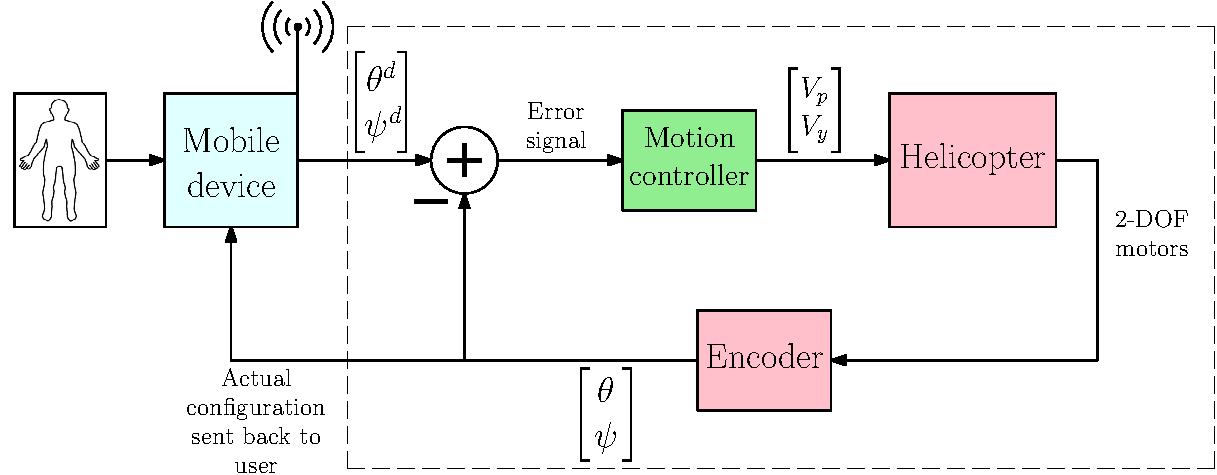
\includegraphics[height=.15\textheight,width=.92\textwidth,keepaspectratio=true]{figs/ipe/algorithmFramework}}
    \caption{A desired orientation is given by a user.  The difference between this input and the actual position is calculated.  The controller the calculates the proper amount of voltage to apply to the DC motors.}
    \label{fig:algorithmFramework}
\end{figure}
%\end{itemize} 
\vskip -1cm
\begin{enumerate}
    \item Employ state-space representation of 2-DOF helicopter:
    \begin{align*}
        \dot{\mathbf{x}} = \mathbf{A}\mathbf{x} + \mathbf{B}\mathbf{u}
    \end{align*}
    \item Use state feedback law
    \begin{center}
        \vskip -1cm
        $\mathbf{u} = -\mathbf{K}\mathbf{x}$
    \end{center}
    \vskip -1cm
    to minimize the quadratic cost function:
    \begin{align*}
        J(\mathbf{u}) = \int_0^\infty (\mathbf{x}^T\mathbf{Q}\mathbf{x} + \mathbf{u}^T\mathbf{R}\mathbf{u} + 2\mathbf{x}^T\mathbf{N}\mathbf{u})\mathrm{dt}
    \end{align*}
    \item Find the solution $\mathbf{S}$ to the Riccati equation
    \begin{align*}
        \mathbf{A}^T\mathbf{S}+\mathbf{SA}-(\mathbf{SB}+\mathbf{N})\mathbf{R}^{-1}(\mathbf{B}^T\mathbf{S}+\mathbf{N}^T)+\mathbf{Q}=0
    \end{align*}    
    \item Calculate gain, $\mathbf{K}$
    \begin{center}
        $\mathbf{K}=\mathbf{R}^{-1}(\mathbf{B}^T\mathbf{S}+\mathbf{N}^T)$
    \end{center}
\end{enumerate}

%\vskip -2.5cm
\end{block}

%-----------------------------------------------------------
% LQG
%-----------------------------------------------------------

\begin{block}{Optimal Noise Resistant Control Algorithm}
\vskip -1cm
\begin{itemize}
    \item Utilizes gain calculated in LQR
    \item Added Kalman filter to reduce external disturbances to the system
%    \begin{subequations}
%        \small
%        \begin{align}
%            & some eq = x\\
%            & some eq = y\\
%            & some eq = z
%        \end{align}
%    \label{eq:LQG_EQ}
%    \end{subequations}
\end{itemize} 
%\todo[inline]{Insert Dr. Miah's LQG image from his slides here}
\begin{figure}
    \centering
    % \missingfigure{Insert figure.}
    \fcolorbox{gray!10}{gray!10}{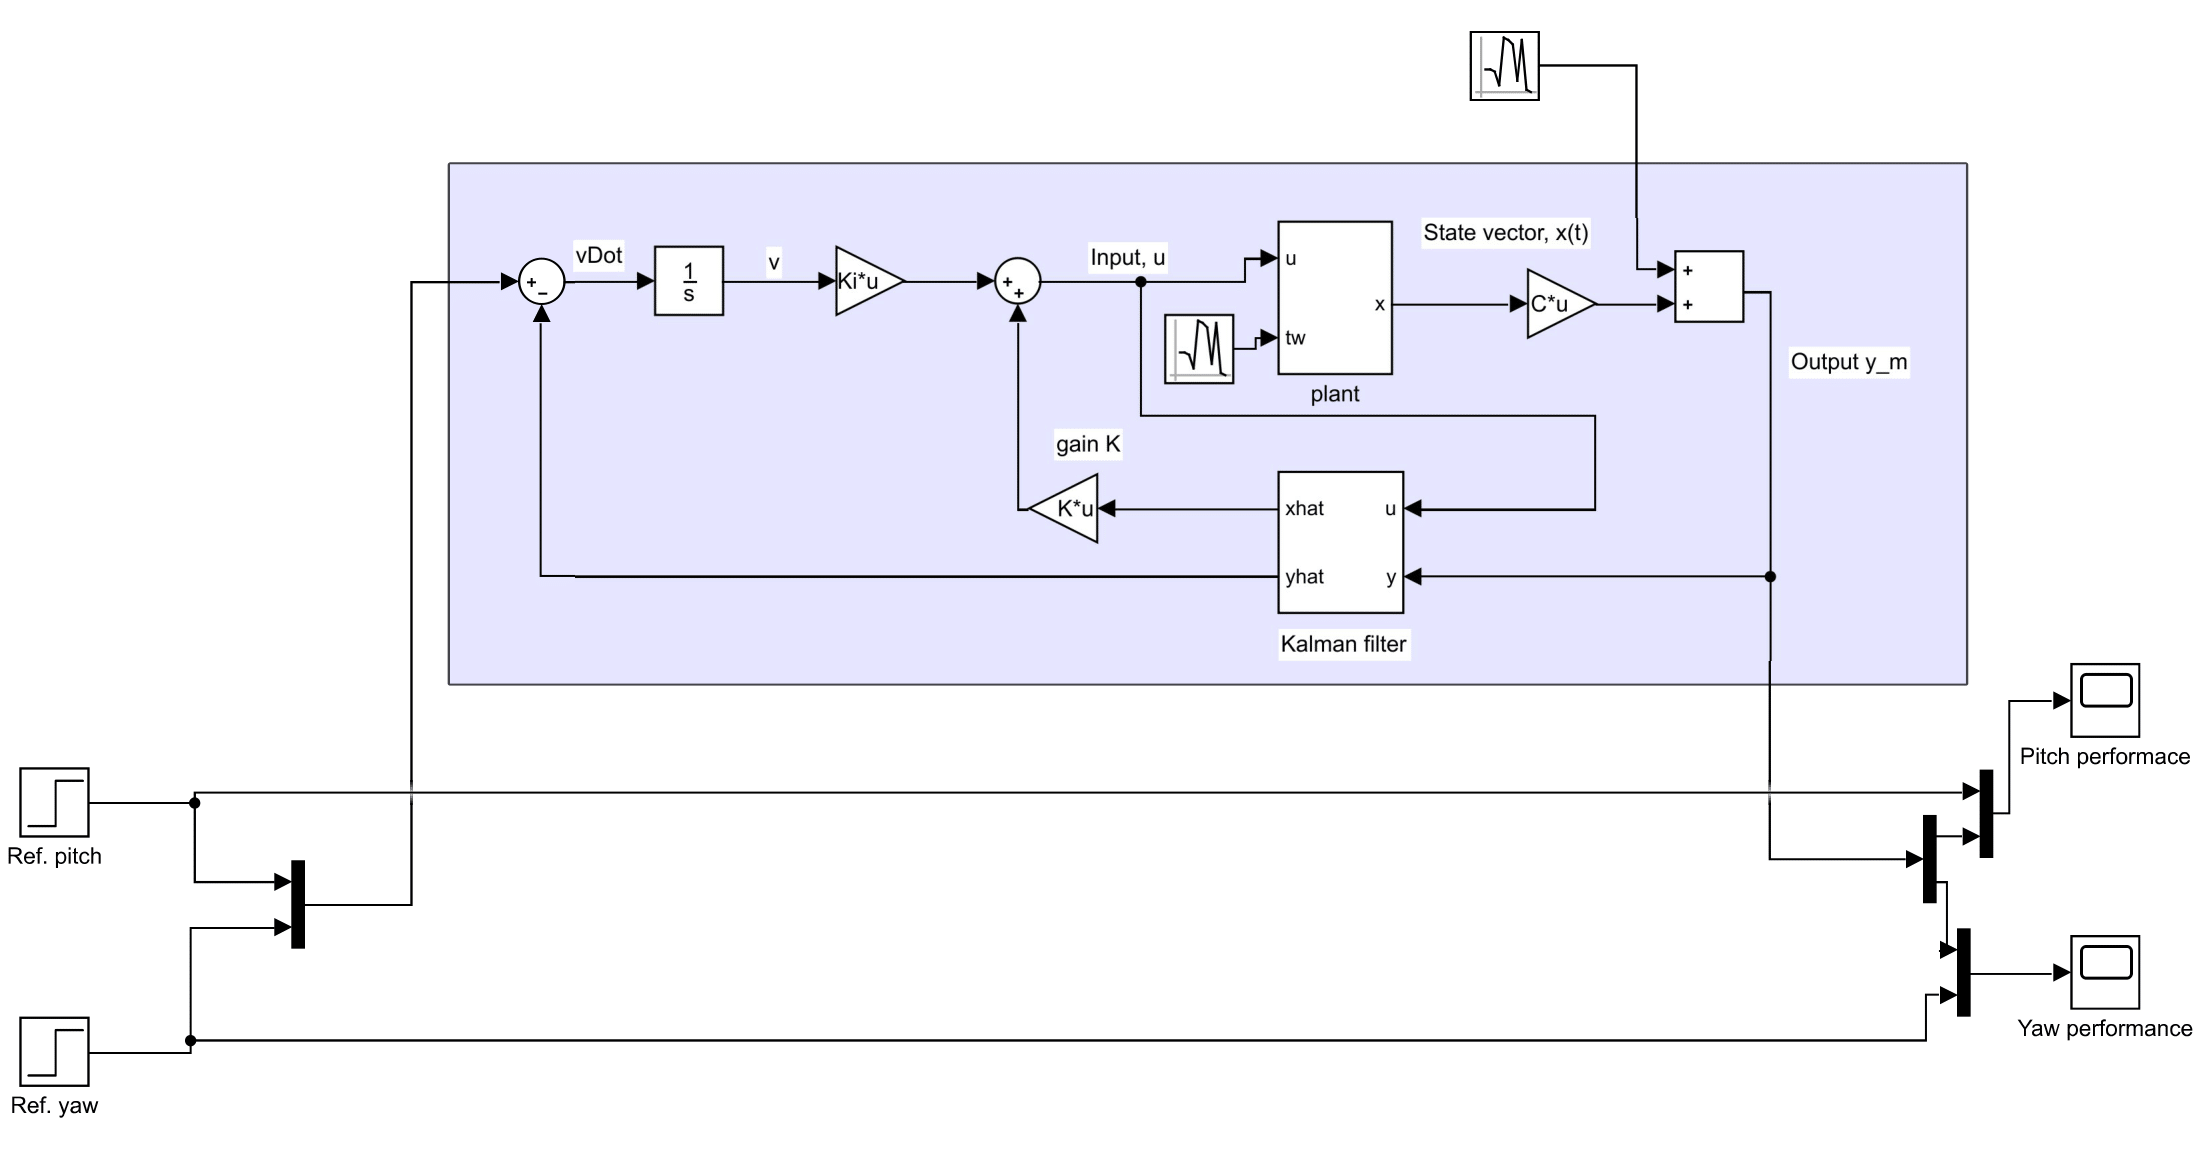
\includegraphics[width=1.05\textwidth,keepaspectratio=true]{figs/img/LQG_SimulinkResize.png}}
    \caption{Noise resistant 2-DOF helicopter model.}
    \label{fig:LQGModel}
\end{figure}

%\vskip -2.5cm
\end{block}



\end{column} % End of second column

\begin{column}{\sepwid}\end{column} % Empty spacer column

\begin{column}{\onecolwid} % The third column
%-----------------------------------------------------------
% ADP
%-----------------------------------------------------------

\begin{block}{Reinforcement Learning Algorithm}
\vskip -1cm
\begin{itemize}
    %\item Reinforcement learning based approach
    \item Uses neural network based on difference between desired and actual orientation to determine optimal gain
    %\item Unlike LQR, ADP operates only in discrete-time and calculates new gains as the system is running
%    \begin{subequations}
%        \small
%        \begin{align}
%            & some eq = x\\
%            & some eq = y\\
%            & some eq = z
%        \end{align}
%    \label{eq:ADP_EQ}
%    \end{subequations}
\end{itemize} 
%\begin{enumerate}
%    \item Apply input to the system and calculate error e(k) at time k
%    \item Use Euler's method to convert the error model into discrete-time and record data every $\tau \sec$
%    \begin{center}
%        $e_{k+1}=f(e_k)+G(e_k)u_k$
%    \end{center}
%    \item 
%    %\item Minimize the cost function
%    %\begin{center}
%        $J(u)=\sum_{k=0}^{\infty} e_k^TQe_k+u_k^TRu_k$
%    %\end{center}
%    %\item Define value function
%    %\begin{center}
%        $V(e_k)=$
%    %\end{center}    
%    \item Solve for gain, K
%    \begin{center}
%        $K=0.5R^{-1}B^TP$
%    \end{center}
%\end{enumerate}

\begin{figure}
    \centering
    \fcolorbox{gray!10}{gray!10}{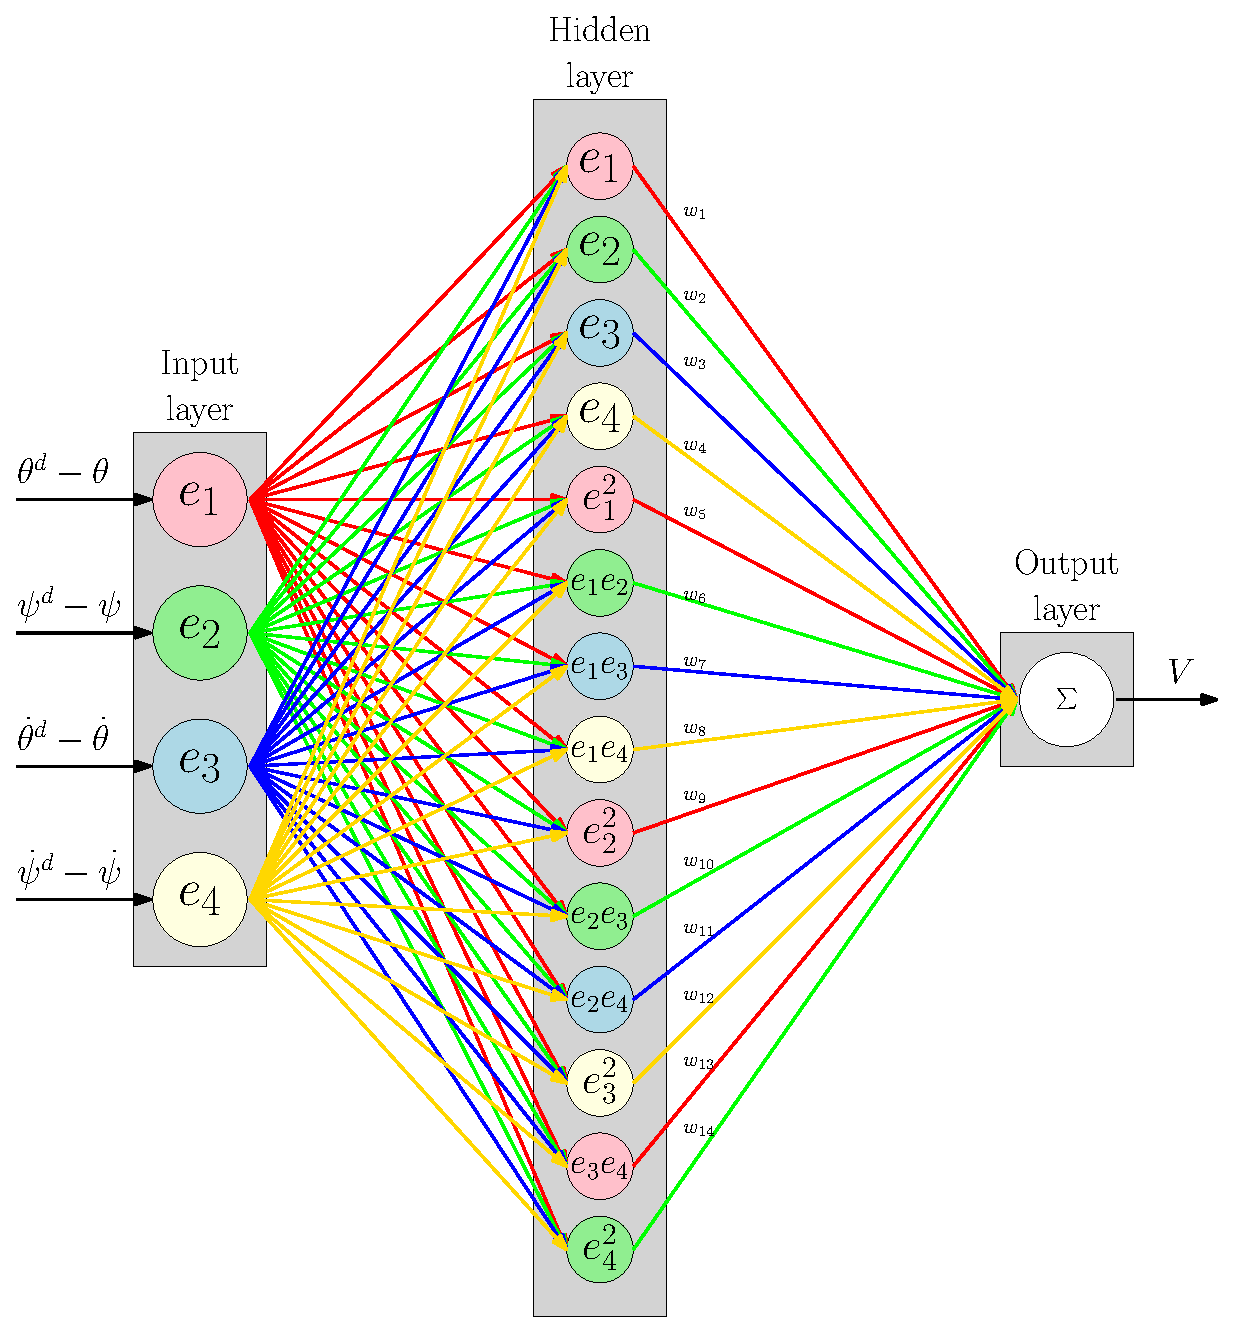
\includegraphics[width=.9\textwidth,keepaspectratio=true]{figs/ipe/ADP_Neural_Network.eps}}
    \caption{ADP Neural Network}
    \label{fig:NeuralNetwork}
\end{figure}



\vskip 1.5cm
%(1) t = kτ where τ is given
%(2)Advance the system by applying determined inputs to the system and measure system states
%(3)Calculate state error as e[k] = xref[k] − x[k], save state error
%(4) If t 6= T, increment k and start at (1)
%(5) If t = T, update K using collected error data
%(5a)Use error states since last update of K as inputs to the neural network
%(5b)Recursively determine wc values for each of the instances
%(5c)Approximate new wc value using regression analysis of the individually calculated wc values
%(6)Calculate new K using wc values
%(7) Increment k and start at (1)


\vskip -2.5cm
\end{block}
%-----------------------------------------------------------
% Subsystem Block Diagram
%-----------------------------------------------------------
%\begin{block}{Subsystem Block Diagram}
%\begin{figure}
%    \centering
%        \missingfigure{Insert figure.}
%    % \boxed{\includegraphics[width=.92\textwidth,keepaspectratio=true]{figs/ipe/subsystemBlockDiagramAlternate2}}
%    \label{fig:subsystem}
%\end{figure}
%\end{block}

%-----------------------------------------------------------
% SIMULATION RESULTS
%-----------------------------------------------------------

\begin{block}{Simulation Results}
\vskip -1cm
%\begin{itemize}
%    \item \todo[inline]{add LQR and LQG simulation results}
%\end{itemize}

%Before implementing the algorithm, it was simulated using the industry standard robot simulator V-REP. With numerous robot models available, V-REP is able to accurately and consistently produce like those expected in real--world scenarios. Preliminary simulation results can be seen in Fig.~\ref{fig:vrepResults}.

\begin{figure}
    \centering
    \subfigure[][]{
    %\missingfigure{Insert figure.}
    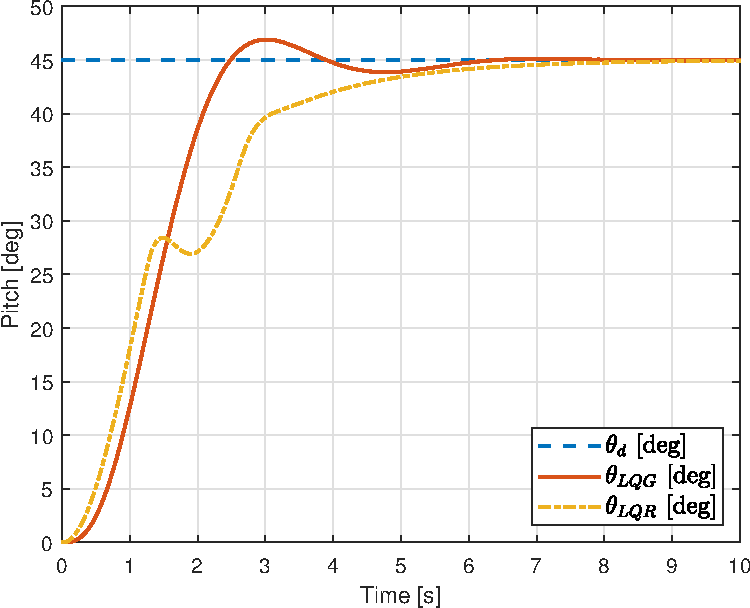
\includegraphics[width=.46\textwidth,keepaspectratio=true]{figs/matlab/LQG_PIvLQR_PI_Sim/Pitch}
    \label{fig:simStepPitch}
    }
    \subfigure[][]{
    %\missingfigure{Insert figure.}
    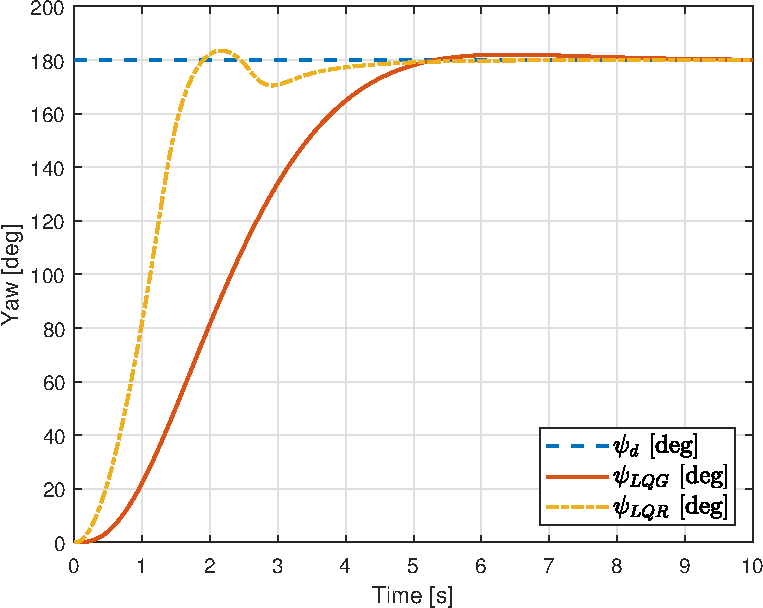
\includegraphics[width=.46\textwidth,keepaspectratio=true]{figs/matlab/LQG_PIvLQR_PI_Sim/Yaw}
    \label{fig:simStepYaw}
    }
    \subfigure[][]{
    %\missingfigure{Insert figure.}
    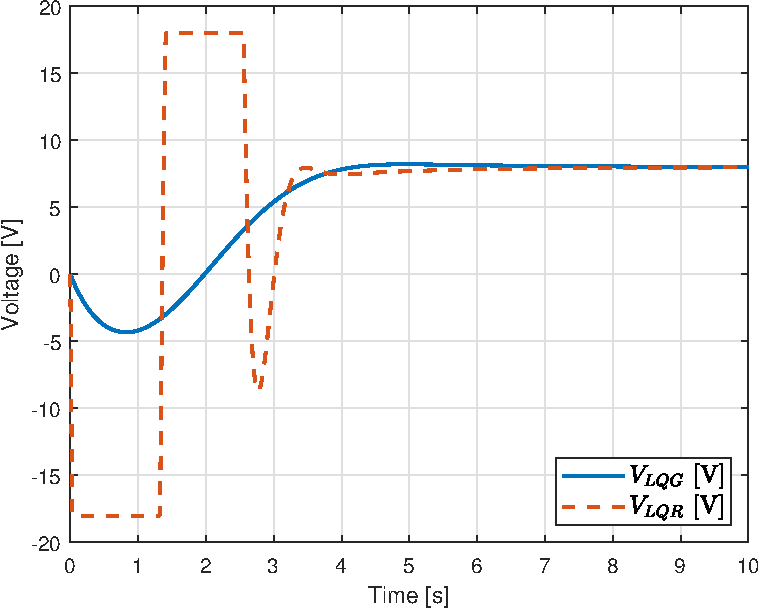
\includegraphics[width=.46\textwidth,keepaspectratio=true]{figs/matlab/LQG_PIvLQR_PI_Sim/Pitch_Volt}
    \label{fig:simPitchVolt}
    }
    \subfigure[][]{
    %\missingfigure{Insert figure.}
    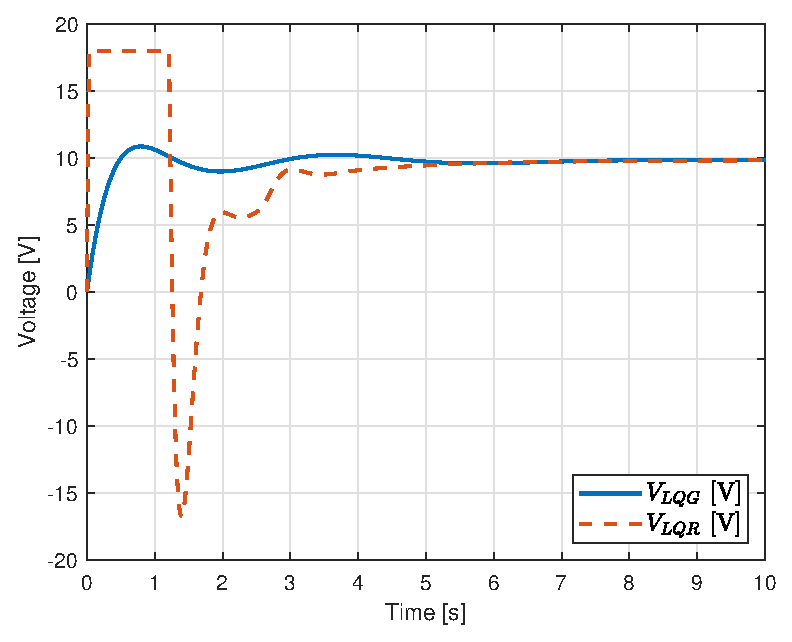
\includegraphics[width=.46\textwidth,keepaspectratio=true]{figs/matlab/LQG_PIvLQR_PI_Sim/Yaw_Volt}
    \label{fig:simYawVolt}
    }
    \caption{A comparison between LQG and LQR control for a step input is shown for \subref{fig:simStepPitch}~the~main~rotor and \subref{fig:simStepYaw}~the~tail~rotor and the corresponding voltages in \subref{fig:simPitchVolt}~and~\subref{fig:simYawVolt}}
    \label{fig:simResults}
\end{figure}
\vskip -2cm
\end{block}


\end{column} % End of third column

\begin{column}{\sepwid}\end{column}

\begin{column}{\onecolwid} % The fourth column

%-----------------------------------------------------------
% EXPERIMENTAL RESULTS
%-----------------------------------------------------------

\begin{block}{Experimental Results}
\vskip -1cm
%\begin{itemize}
%    \item ADP Algorithm
%\end{itemize}
\begin{figure}
    \centering
    \fcolorbox{gray!10}{gray!10}{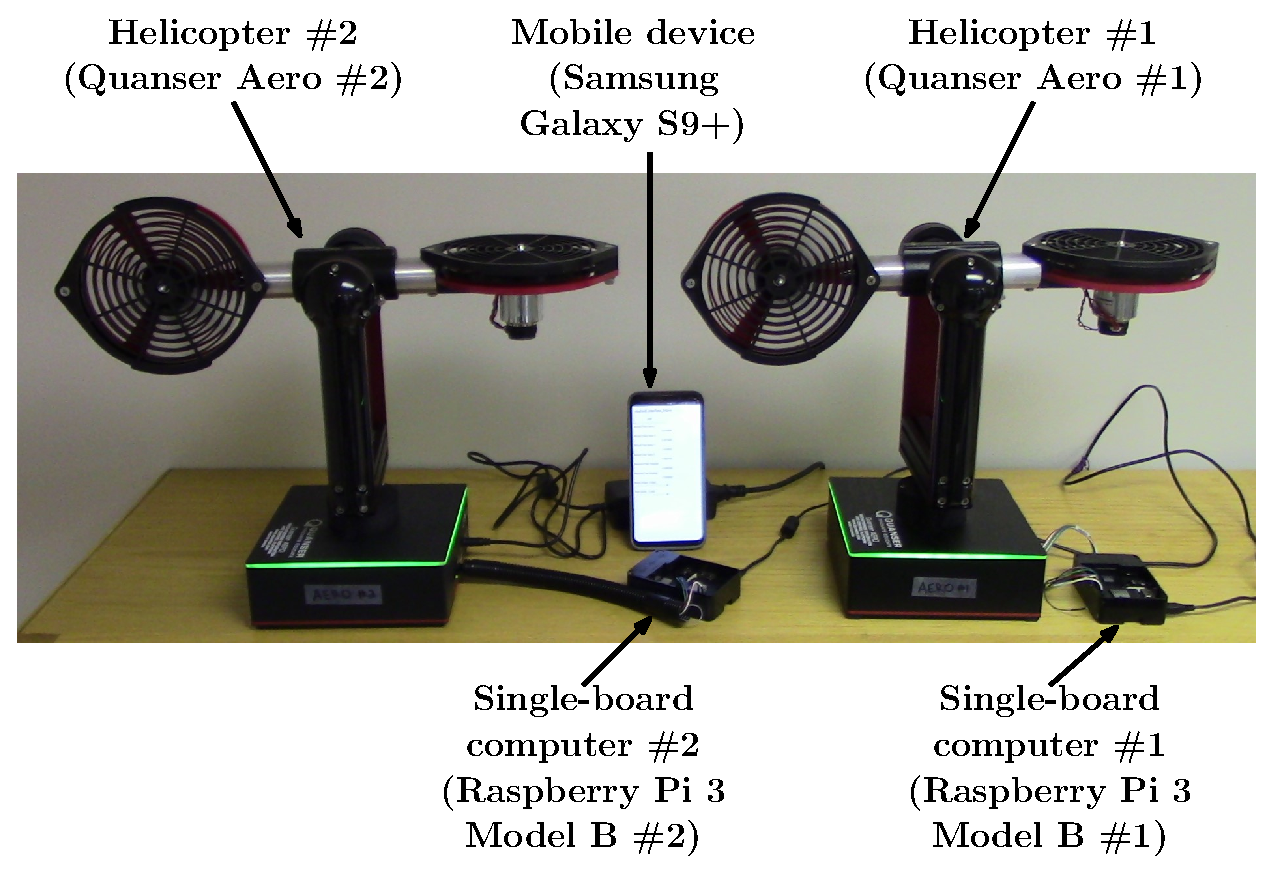
\includegraphics[height=.15\textheight,width=.9\textwidth,keepaspectratio=true]{figs/ipe/setup.eps}}
    \caption{Experimental Setup}
    \label{fig:Setup}
\end{figure}

\begin{figure}
    \centering
    \subfigure[][]{
    %\missingfigure{Insert figure.}
    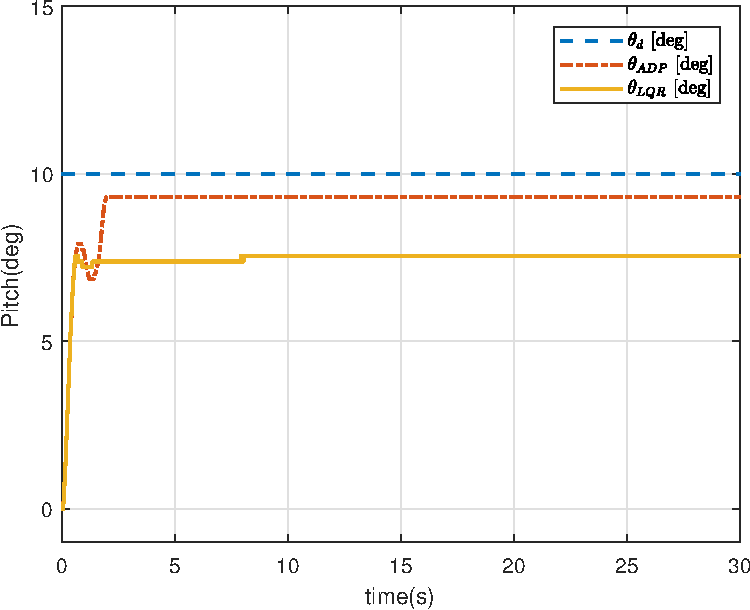
\includegraphics[width=.46\textwidth,keepaspectratio=true]{figs/matlab/ADPvLQR_P_USB/Pitch_ADP_LQR}
    \label{fig:stepPitchADP}
    }
    \subfigure[][]{
    %\missingfigure{Insert figure.}
    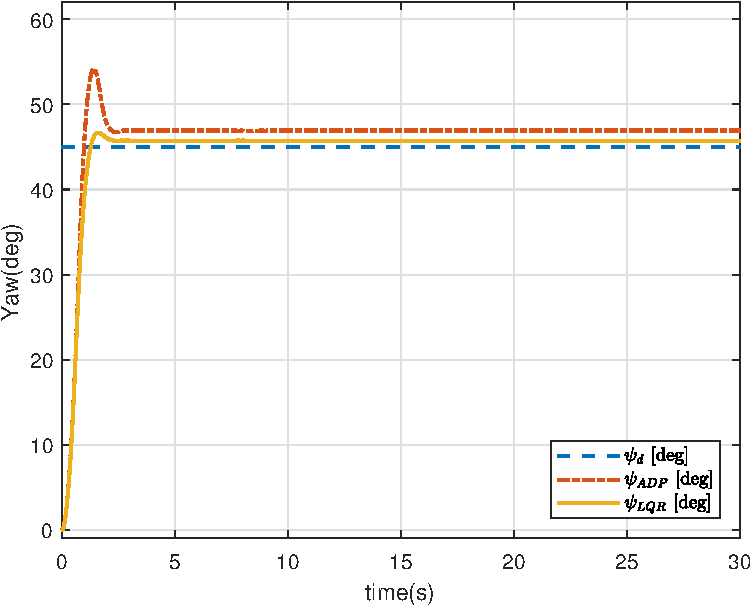
\includegraphics[width=.46\textwidth,keepaspectratio=true]{figs/matlab/ADPvLQR_P_USB/Yaw_ADP_LQR}
    \label{fig:stepYawADP}
    }
    \caption{ADP experimental results for \subref{fig:stepPitchADP}~the~main~rotor and \subref{fig:stepYawADP}~the~tail~rotor given a step input}
    \label{fig:ADP_Results}
\end{figure}
%\begin{itemize}
%    \item Comparison between different controller architectures (proportional controller and proportional controller with integral term)
%\end{itemize}
\vskip -.5cm

\begin{figure}
    \centering
    \subfigure[][]{
    %\missingfigure{Insert figure.}
    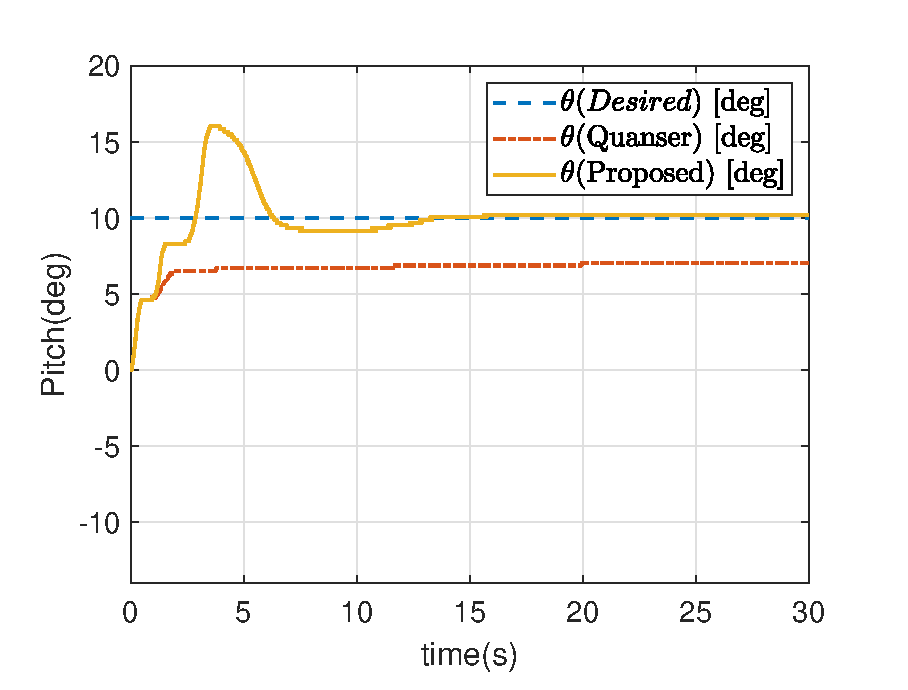
\includegraphics[width=.46\textwidth,keepaspectratio=true]{figs/matlab/LQR_PIvLQR_P_USB/step/Pitch_LQR_RMSE}
    \label{fig:stepPitch}
    }
    \subfigure[][]{
    %\missingfigure{Insert figure.}
    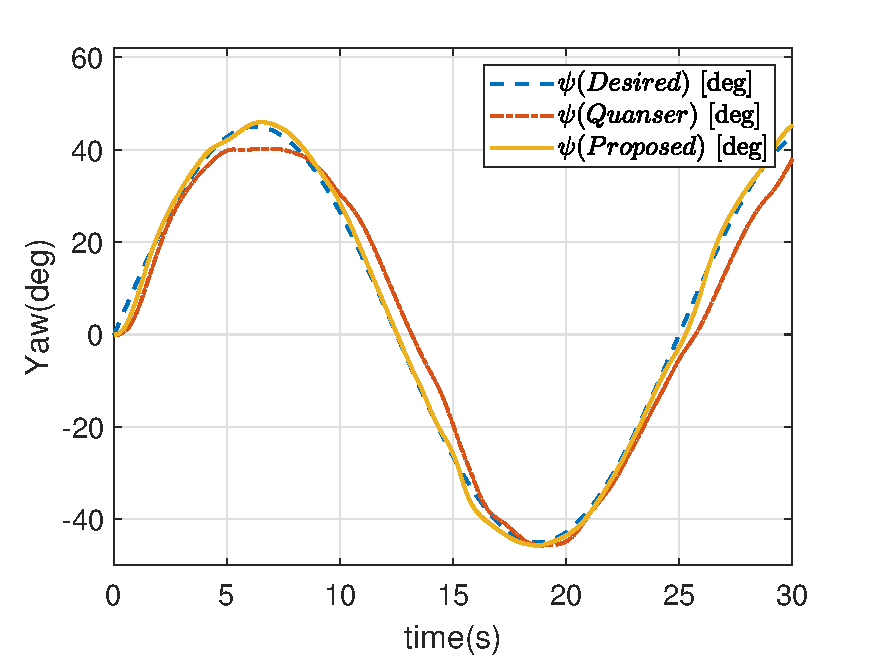
\includegraphics[width=.46\textwidth,keepaspectratio=true]{figs/matlab/LQR_PIvLQR_P_USB/step/Yaw_LQR_RMSE}
    \label{fig:stepYaw}
    }
    \caption{Comparison between P and PI control for a step input is shown for \subref{fig:stepPitch}~the~main~rotor and \subref{fig:stepYaw}~the~tail~rotor}
    \label{fig:expResults}
\end{figure}
\vskip -2cm
\end{block}

\begin{figure}
  \centering
  \subfigure[][]{
  \label{fig:time0}
  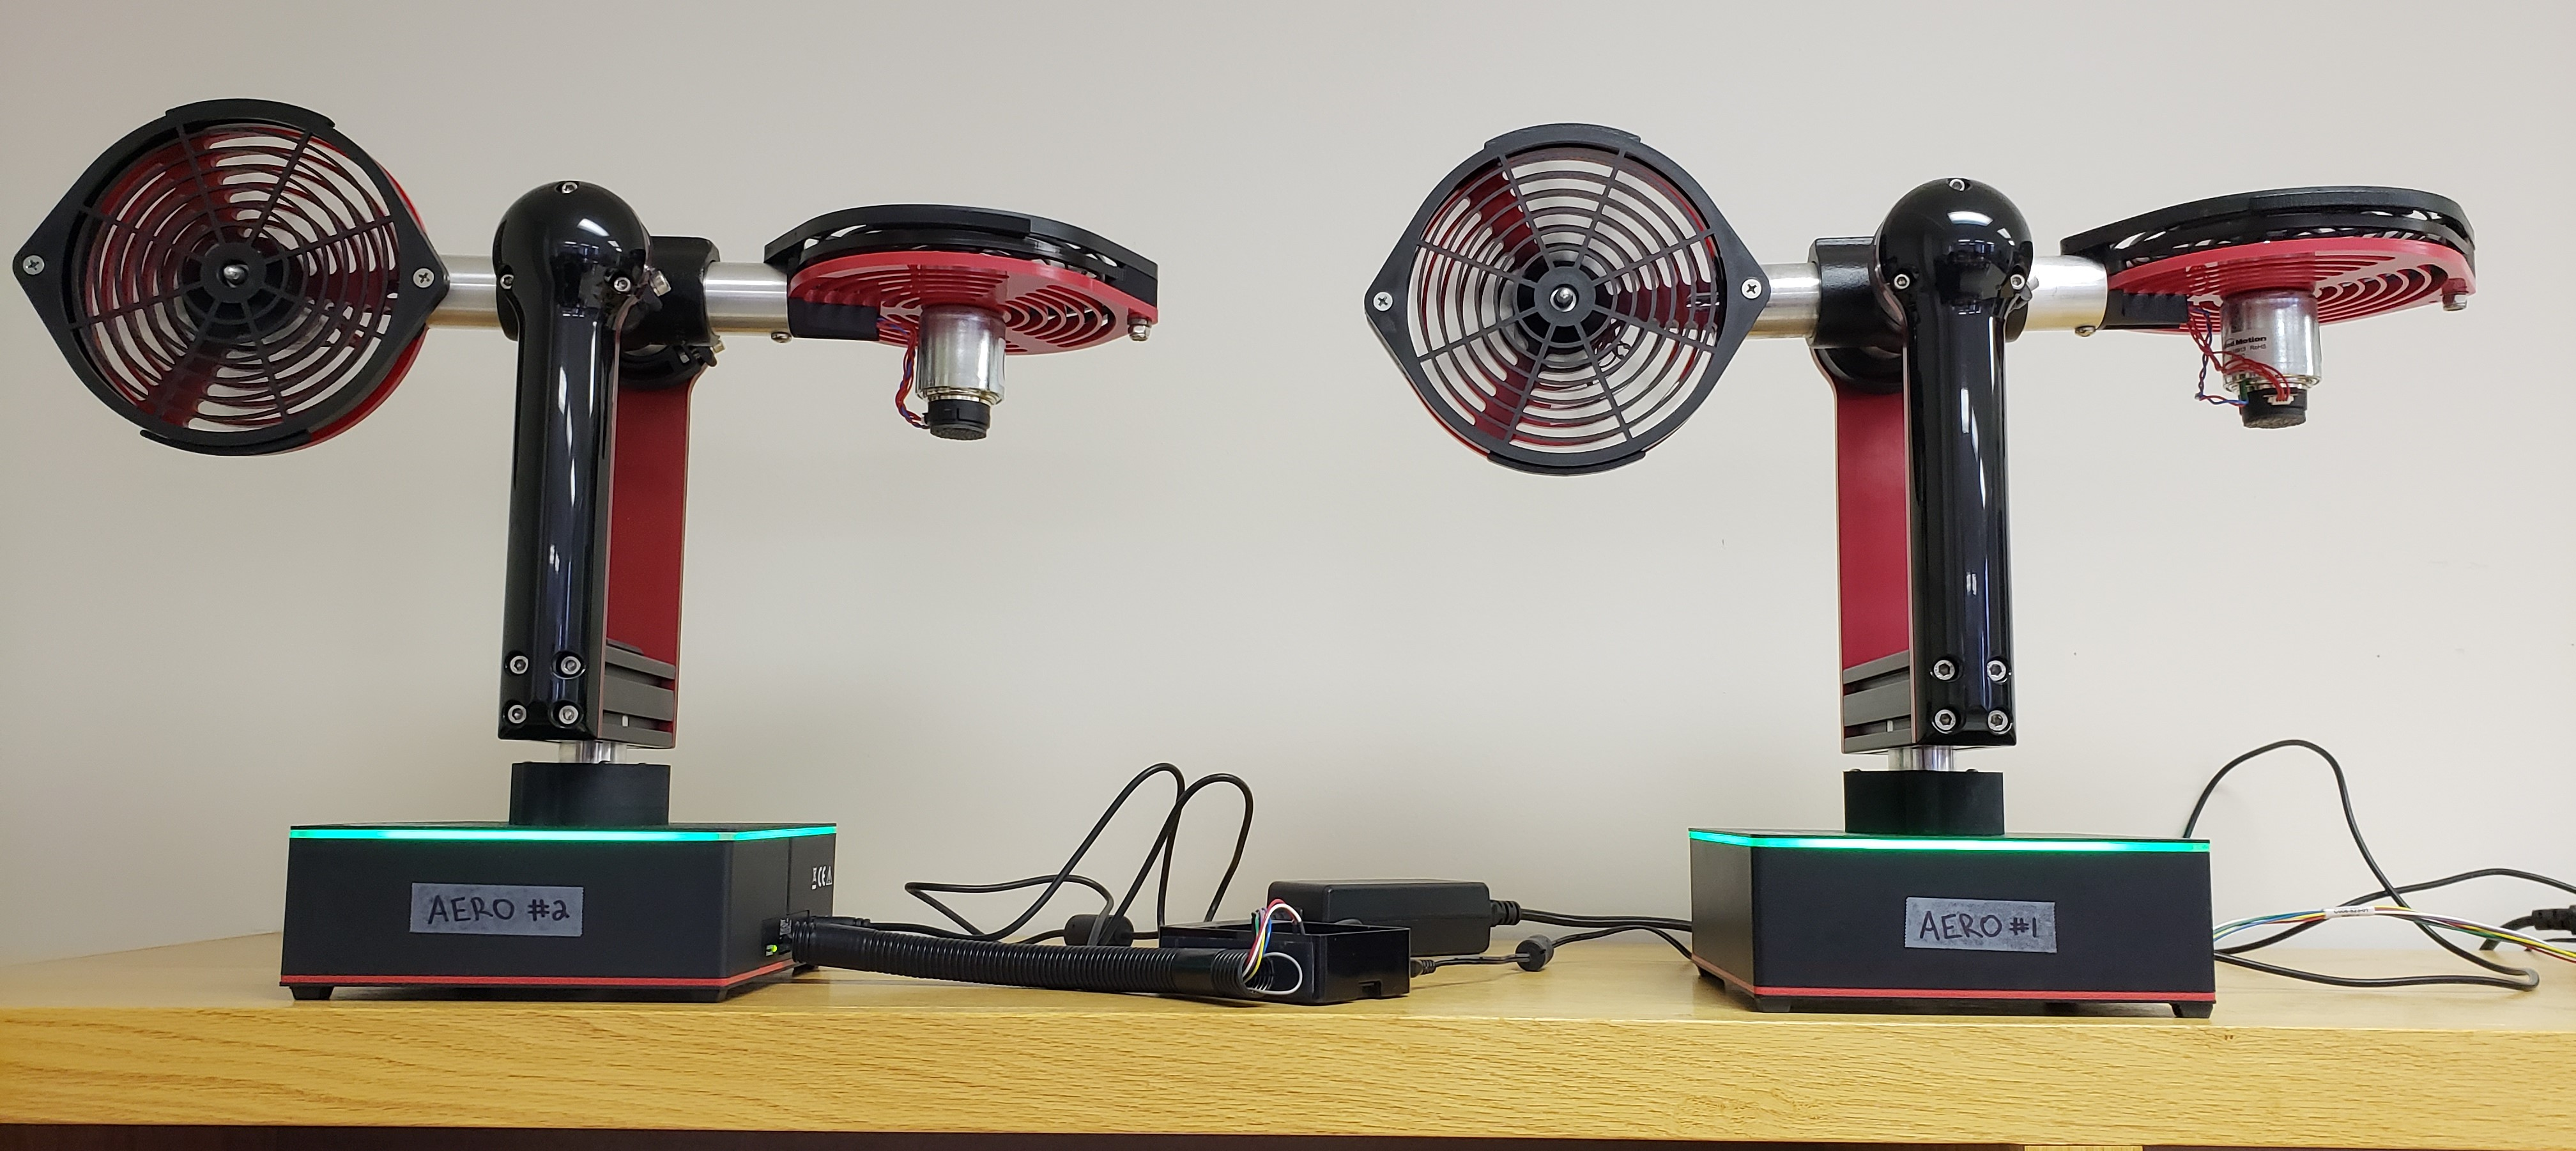
\includegraphics[width=0.4\textwidth]{figs/img/timeEquals0.jpg}
  }
  \subfigure[][]{
  \label{fig:time10}
  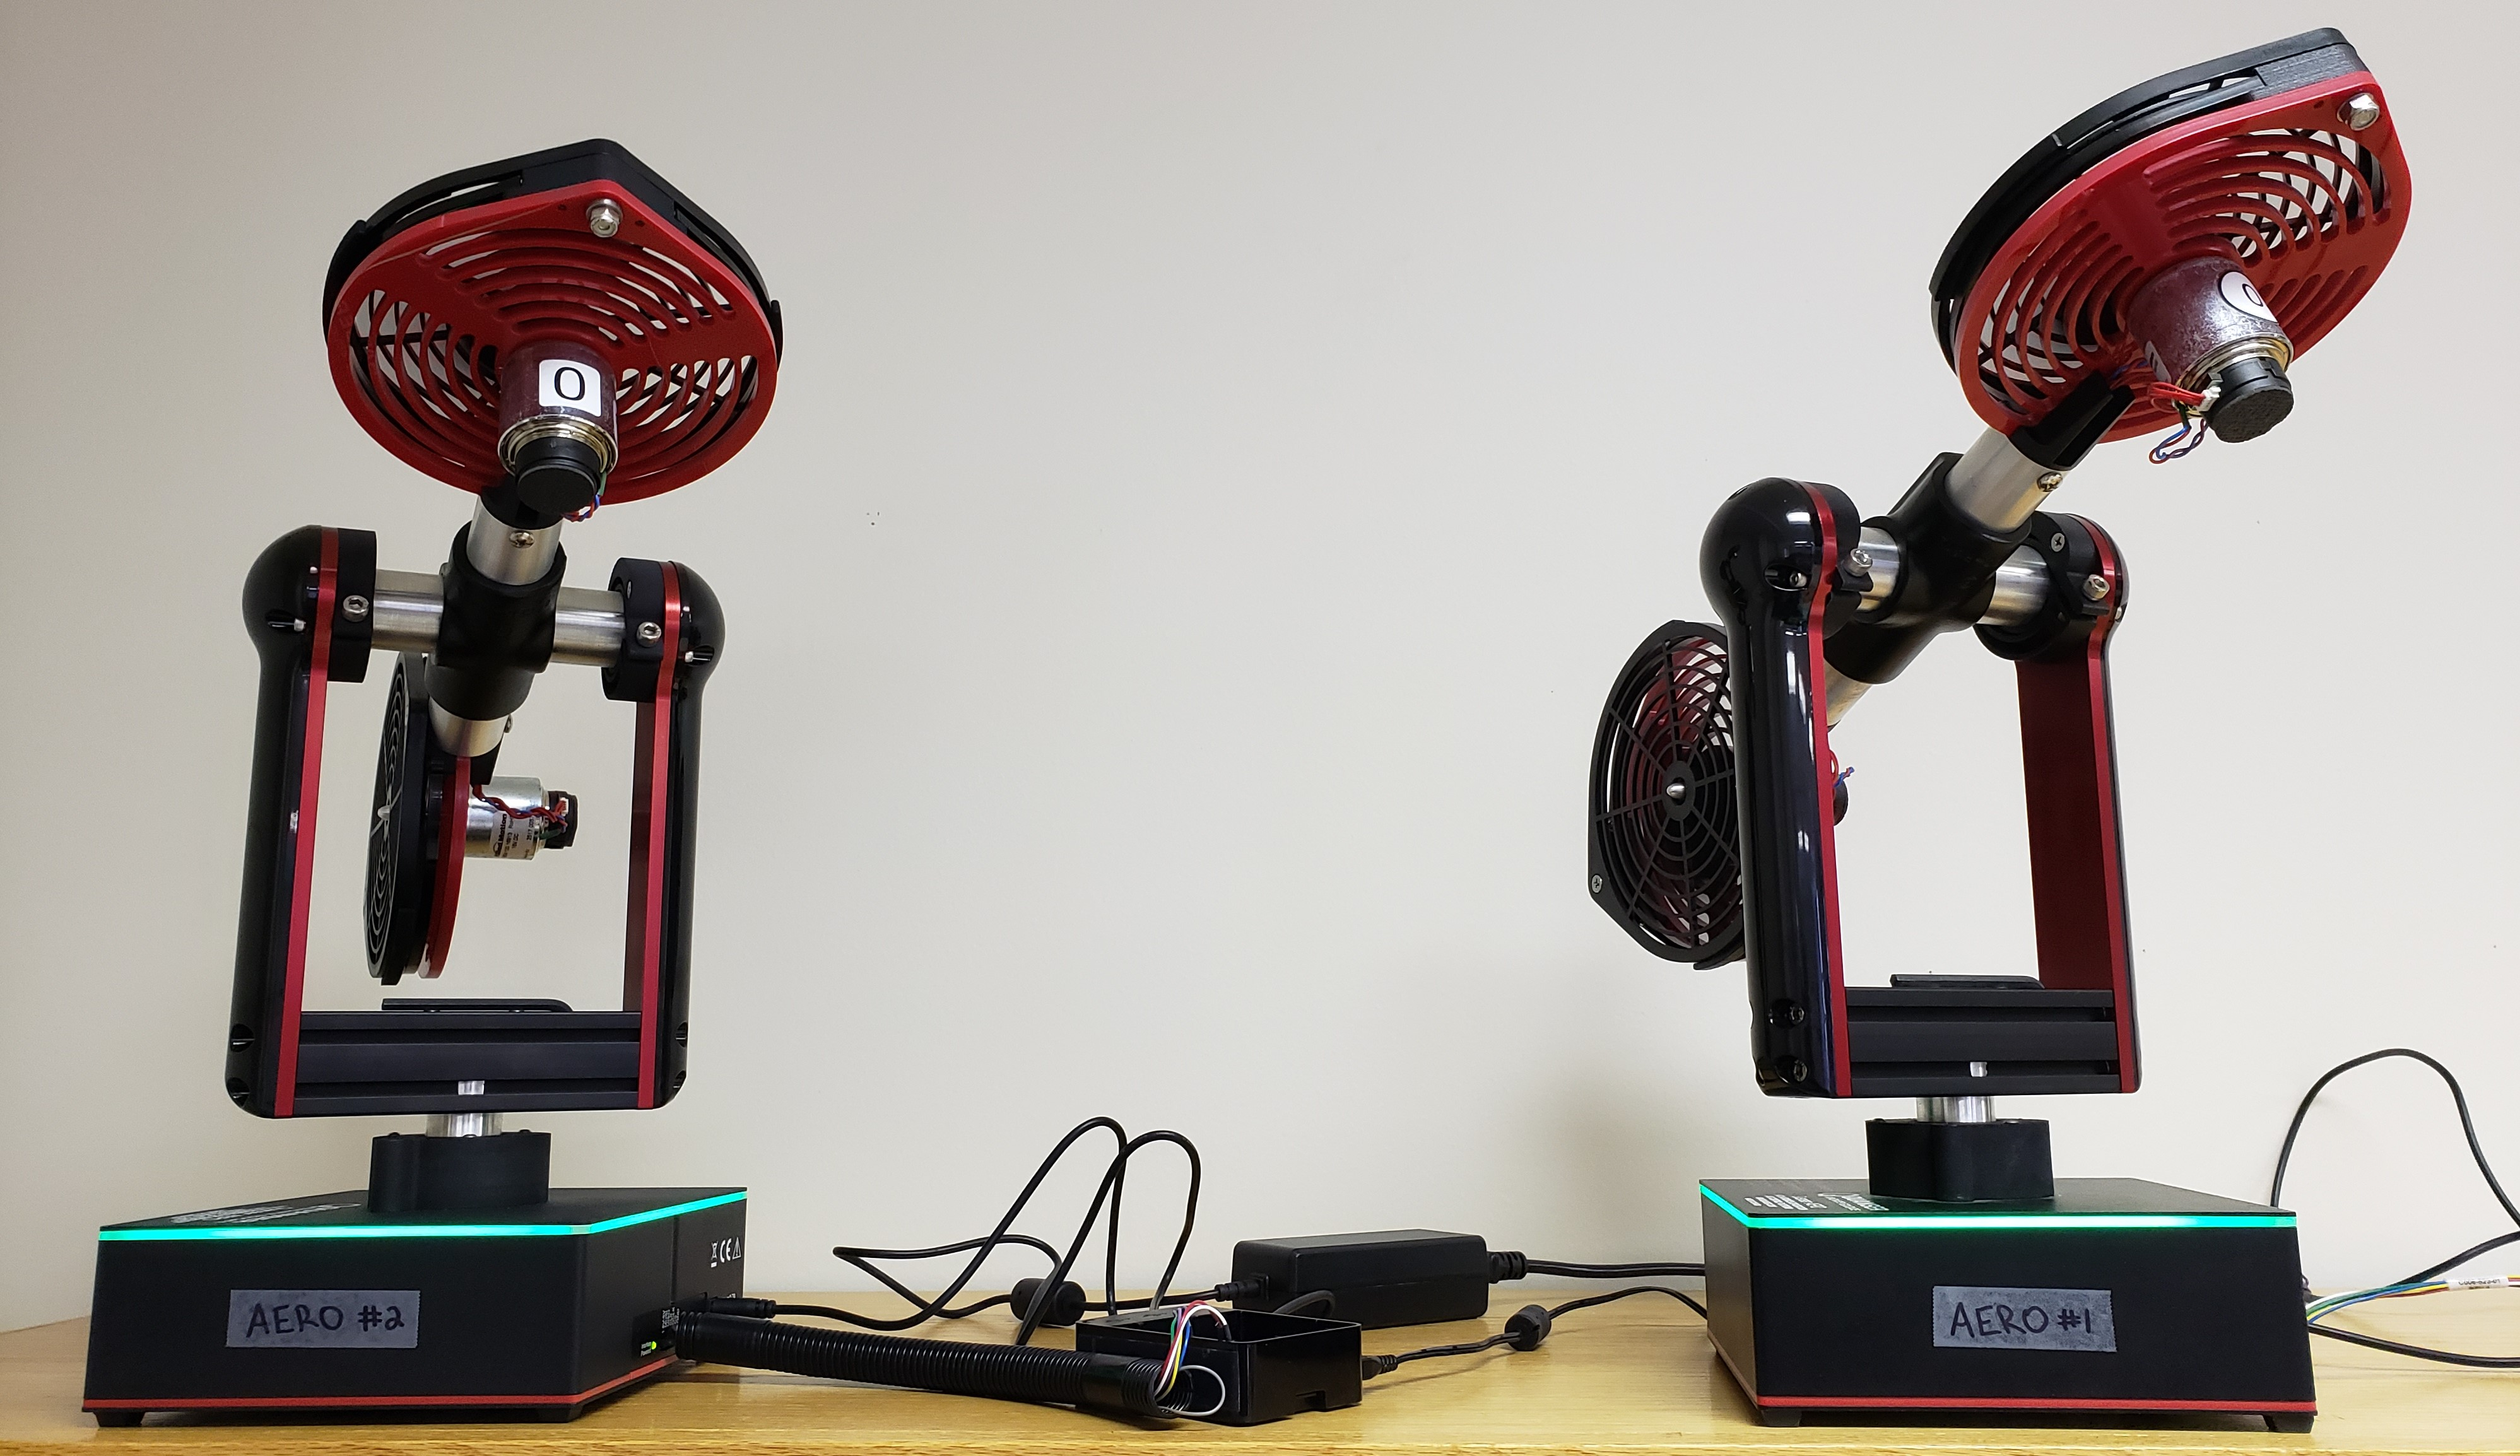
\includegraphics[width=0.4\textwidth,height=0.057\textheight]{figs/img/timeEquals10_2}
  }  
  \caption{\subref{fig:time0} Time = 0~and~\subref{fig:time10} Time = 10}
  \label{fig:posistionAtTime}
\end{figure}

%\begin{block}{Conclusion}

%As seen in the experimental results, this system brings moderate accuracy considering its implementation. With a total cost of around \$140 for the system mounted on the mobile robot and around \$23 for the beacons, this system is much more attainable for those conducting research in mapping and localization algorithms and inexpensive to scale to commercial applications.

%\end{block}

%-----------------------------------------------------------
% Conclusion and Future Work
%-----------------------------------------------------------

\begin{alertblock}{Conclusion and Future Work}
\begin{itemize}
    \item Model-based reinforcement learning technique (ADP)  is useful when system model is unknown
   % \item PI controller greatly reduces steady-state error, however increases overshoot and settling time
    \vskip .75cm
    \item Implement PI controller for ADP algorithm
    \item Use digital compass to increase accuracy of orientation and help identify initial position
\end{itemize}


\end{alertblock}

\end{column} % End of the fourth column

\end{columns} % End of all the columns in the poster

\end{frame} % End of the enclosing frame

\end{document}

%%% Local Variables:
%%% mode: latex
%%% TeX-master: t
%%% End:
